\chapter{Introduction\label{chap:introduction}}
\section{Small molecule drug design\label{sec:drug-design}}

The discovery of novel drugs has significantly contributed to the improvement of human health and
well-being. There is a continuous demand for new drugs to expand the range of treatable diseases,
improve the efficacy of existing treatments, and respond to the emergence of new health challenges.

Small molecule drugs constitute the majority of medicines in use, accounting for approximately 90\%
of global sales \citep{makurvetBiologicsVsSmall2021}. These molecules, typically defined as having a
molecular weight of less than 900 Da, offer several advantages. They are generally stable, do not
require specialized storage conditions, and can be conveniently administered orally. Moreover, they
are relatively inexpensive to produce and can be easily synthesized in large quantities
\citep{southeyIntroductionSmallMolecule2023}.

For a small molecule to be considered a viable drug candidate, it must fulfill a range of properties:
\begin{itemize}
    \item \textbf{On-target activity:} The molecule must be active against the desired biological target to exhibit
          the intended therapeutic effect. At the molecular level, this means binding to the target or
          modulating its activity in the desired manner.
    \item \textbf{Specificity:} The molecule should demonstrate high specificity, selectively
          interacting with the intended target while minimizing undesirable off-target interactions. Such
          selectivity is crucial to prevent adverse side effects and maintain the drug's safety and efficacy
          profile.
    \item \textbf{Toxicity:} The absence of toxic effects is essential, as the molecule must be
          well-tolerated and free from potential harmful side effects. Toxicity can arise from various
          factors, including off-target interactions, metabolic byproducts, or allergic reactions.
    \item \textbf{Pharmacokinetics:} The molecule must possess favorable pharmacokinetic properties,
          encompassing adsorption, distribution, metabolism, and excretion (ADME). These properties determine
          how the molecule is absorbed into the body, distributed throughout, metabolized, and ultimately
          excreted. They are crucial for ensuring the molecule reaches its target effectively and is processed
          safely by the body.
    \item \textbf{Synthesizability:} The molecule must be synthesizable in a cost-effective manner to be
          practically viable for large-scale production.
\end{itemize}

In addition to these properties, the molecule must be novel and not infringe on existing patents.
While this is not inherently necessary for a drug's efficacy, it represents a significant practical
consideration in the pharmaceutical industry.

The primary challenge in drug discovery lies in identifying a molecule that satisfies all these
criteria simultaneously. The development of a new drug is a complex and expensive process, which can
take 12-15 years and cost estimates range between \$1.8-2.5 billion \citep{hughesPrinciplesEarlyDrug2011,paulHowImproveProductivity2010,dimasiInnovationPharmaceuticalIndustry2016}.

\subsection{The drug discovery pipeline}
\begin{figure}
    \centering
    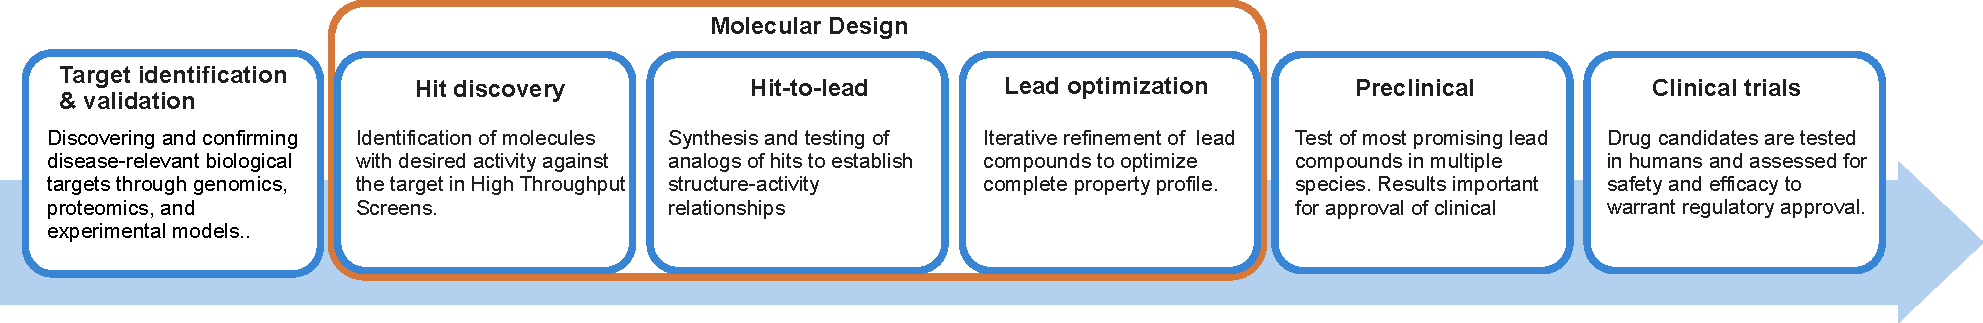
\includegraphics[width=\textwidth]{figures/drug-discovery-pipeline_v2.pdf}
    \caption{The drug discovery pipeline consists of several stages, ranging from target identification
        and validation to clinical trials. Molecular design (orange box) aims at identifying
        molecules with desired property profiles. This phase is particularly amenable to
        computational methods, which can accelerate the discovery process and reduce the cost of
        experimental testing\label{fig:drug-discovery-pipeline}}.
\end{figure}

The drug discovery process typically comprises several distinct stages. We outline the stages
described in \citet{hughesPrinciplesEarlyDrug2011} and \citep{umscheidKeyConceptsClinical2011} here and illustrate them in \Cref{fig:drug-discovery-pipeline}:
\begin{itemize}
    \item \textbf{Target Identification and Validation:} The drug discovery process begins with
          the identification of a biological target, such as a protein or nucleic acid, that is
          believed to be associated with a disease. Then target validation is performed using
          various experimental techniques to increase confidence that the target is indeed worth
          pursuing.
    \item \textbf{Hit Discovery:} The hit discovery stage aims at finding "hits", i.e. molecules
          that exhibit activity against the target in a compound screen. Molecules are tested in
          so-called assays, experiments designed to measure the activity of a molecule against the
          target. The screened compound libraries range from large unfocussed libraries tested in
          \ac{HTS} to smaller more focused libraries if there already is some knowledge of promising
          compound classes. Computational models that predict molecular properties and activities
          can be used in \ac{VS}
          \citep{waltersVirtualScreeningOverview1998,shoichetVirtualScreeningChemical2004a} to
          evaluate large compound libraries to prioritize compounds for experimental testing.
    \item \textbf{Hit-to-lead}: This phase aims to develop more potent and selective compounds
          based on the identified hits. This often involves a systematic exploration of the
          structure-activity relationship around the hit molecules.  The hits are further tested on
          their pharmacokinetic properties and toxicity, further narrowing down the number of
          compounds.
    \item \textbf{Lead Optimization:} This phase aims to optimize the properties of the
          lead compounds identified in the hit-to-lead phase. The goal is to maintain the favorable
          properties of the lead compounds while avoiding any unwanted side effects.
    \item \textbf{Preclinical Development:} The most promising lead compounds are then tested in
          preclinical studies, which are typically conducted in animal models. These studies focus
          on exploring efficacy, pharmacokinetics, and toxicology of the drug candidate. The data
          generated during this stage are critical for determining whether the candidate is
          suitable for clinical trials in humans.
    \item \textbf{Clinical Trials:} Drug candidates that pass preclinical development proceed to
          clinical trials, which are conducted in humans and are typically divided into three phases:
          \begin{itemize}
              \item \textbf{Phase I:} The drug is tested in a small group of "healthy" and/or "diseased" people to learn about
                    dosage, safety, and side effects. This phase is usually the first time the drug is tested in humans.
              \item \textbf{Phase II:} In this phase, the efficacy of the drug is tested in a larger
                    group of patients with the disease of interest to study its effectiveness and further investigate safety.
              \item \textbf{Phase III:} This phase involves large-scale testing of the drug's safety
                    and effectiveness comparing it to existing treatments or a placebo.
          \end{itemize}
          The success rates of clinical trials are low, with only about 10\% of drugs that enter clinical
          trials eventually being approved by regulatory agencies. More specifically, the success rates in
          Phase I/II/III are 63\%, 31\%, 58\% which translates to 63\%, 19.5\% and 11.3\% of projects that
          make it through the respective stages \citep{mullardParsingClinicalSuccess2016}.
    \item \textbf{Regulatory Approval:} Upon successful completion of clinical trials, the drug is
          submitted for regulatory approval. Agencies such as the U.S. \Ac{FDA} or the \Ac{EMA}
          review the comprehensive data package, including preclinical and clinical trial results.
          If the drug is deemed safe and effective, it receives approval for marketing and
          distribution. The success rate for submissions for regulatory approval is 85\% which
          translates to 9.6\% of all projects that obtain approval
          \citep{mullardParsingClinicalSuccess2016}.
    \item \textbf{Post-Market Surveillance:} Post-market surveillance, or Phase IV studies, are
          conducted to monitor the long-term safety and efficacy of the drug in the general population.
          This stage can reveal rare side effects or long-term risks that were not apparent during
          clinical trials, and it may lead to further modifications, warnings, or even withdrawal of the
          drug from the market.
\end{itemize}

% General strategy
The general strategy of this process is to start with many molecules and then
systematically reduce the number to a few candidates that finally are submitted to clinical trials.
These range from hundreds of thousands to millions of molecules in the hit discovery phase, to hundreds
in the hit-to-lead and lead optimization phases, to finally one to two molecules in the clinical trials \citep{hughesPrinciplesEarlyDrug2011}.
The early stages have lower per molecule costs but higher uncertainty about the success
chances of a molecule. The later stages are more expensive per molecule, but provide more accurate information
whether a molecule is safe and effective in humans.


\subsection{The Design-Make-Test-Analyze cycle}
\begin{figure}
    \centering
    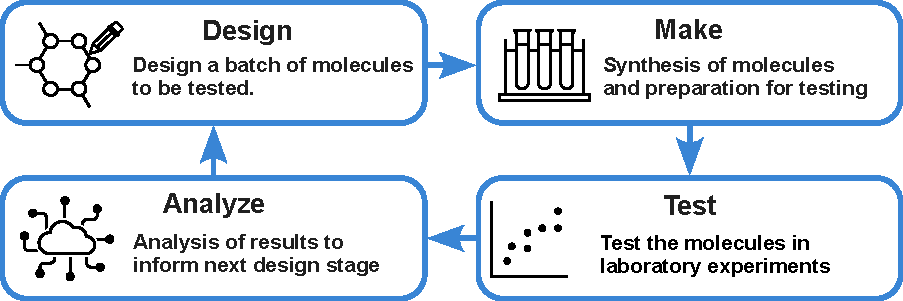
\includegraphics[width=\textwidth]{figures/dmta_cycle_v2.pdf}
    \caption{The Design-Make-Test-Analyze (DMTA) cycle is a key concept in drug discovery. The
        cycle consists of four stages: (a) Design: Molecules to be tested are selected/designed.
        Generative models can be used to design molecules with desired properties. (b) Make: The
        selected molecules are synthesized. Generative models can be used to help in finding
        synthesis routes if not already done in the design stage or if a plan fails. (c) Test:
        The compounds are experimentally evaluated. (d) Analyze: The results of the experiments
        are analyzed and guide the next design stage. \label{fig:dmta-cycle}}
\end{figure}
The hit discovery, hit-to-lead and lead optimization stages usually operate in an iterative manner,
resulting in what is commonly referred to as the \ac{DMTA} cycle \citep{wesolowskiStrategiesPoliticsSuccessful2016}
shown in \Cref{fig:dmta-cycle}. The cycle consists of four stages:
\begin{itemize}
    \item \textbf{Design:} Under consideration of previous experimental results, the molecules to
          be tested are designed. The design generally aims to optimize the desired properties of
          the molecule, but also to explore chemical space to find structure-activity relationships.
    \item \textbf{Make:} The designed molecules are then synthesized and prepared for testing in
          the laboratory. This step requires a synthesis plan that outlines the steps needed to
          make the molecule.
    \item \textbf{Test:} The synthesized molecules are then tested in laboratory experiments to
          measure the properties of interest. This can range from the activity of the molecule
          against a target, to its pharmacokinetic properties, to its toxicity and others.
    \item \textbf{Analyze:} The results of the experiments are analyzed. The obtained insights
          can then be used to guide the design of the next molecules to be tested.
\end{itemize}

The \ac{DMTA} cycle is particularly amenable to computational methods. \Ac{QSPR} models can be used
to predict the properties of molecules in the design phase to guide the selection of molecules
to be tested. \Ac{ML} models can be iteratively refined using new experimental data to
improve their predictive performance. Recently, advances in \ac{DL} have led to an increased
interest in the application of generative models to tackle other aspects of the \ac{DMTA} cycle,
such as the automated design of molecules and the planning of their synthesis.

\section{Generative models in drug discovery}
Generative models are a class of machine learning models that are able to create new data samples.
Recently, advances in \ac{DL} have led to a surge in interest in generative models, with many new
training strategies and model architectures being developed
\citep{bond-taylorDeepGenerativeModelling2022,brownLanguageModelsAre2020,goodfellowGenerativeAdversarialNetworks2014,
    dinhDensityEstimationUsing2017,kingmaAutoEncodingVariationalBayes2013,hoDenoisingDiffusionProbabilistic2020,vaswaniAttentionAllYou2017}.
In drug discovery, these models have opened up new possibilities for tasks that rely on the creation
of novel molecular structures, extending the applicability of \ac{ML}. This thesis focuses on two
key applications of generative models in drug discovery:
\begin{itemize}
    \item \textbf{De Novo Drug Design:} In the field of \ac{DNDD} \citep{schneiderNovoMolecularDesign2013} generative models are used to
          create new molecular structures with desired property profiles. This approach enables
          the efficient exploration of chemical space, without the need for explicit enumeration
          of large compound libraries.
    \item \textbf{Computer-Aided Synthesis Planning:} Generative models are also applied to model
          chemical reactions. These models are then used to find synthesis routes for target
          molecules, addressing a core challenge in drug development.
\end{itemize}

In the remainder of this section, we provide an overview of the key concepts and methods underlying
generative models for molecules, and introduce current challenges in the field.

\subsection{Molecular representations}
\begin{figure}
    \centering
    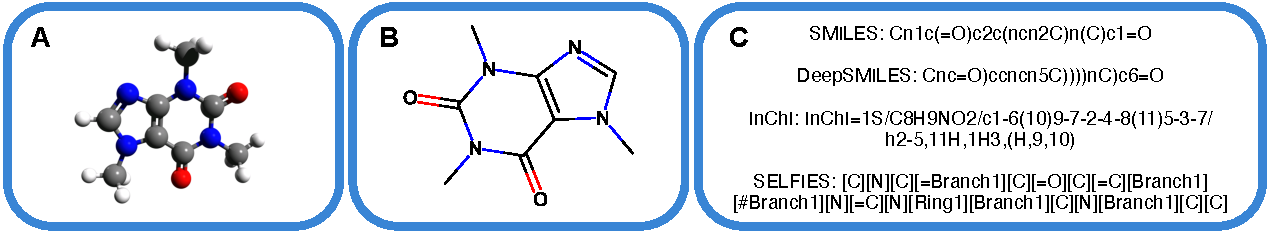
\includegraphics[width=\textwidth]{figures/representations/representations.pdf}
    \caption{Different ways to represent a caffeine molecule. \textbf{A:} The 3D structure of a
        molecule is given by the positions of its atoms in space. This structure is not
        necessarily fixed as some bonds can rotate and/or vibrate (Image source:
        \citep{Caffeine3DStructure2010}). \textbf{B:} The graph representation of the same
        molecule. \textbf{C:} Smiles, DeepSmiles, SELFIES and InChI are line notations that
        linearize the molecule's graph representation.\label{fig:molecular-graph}}
\end{figure}
% shall I add adjacency matrix and node feature matrix here?
Molecules, though fundamentally complex quantum mechanical entities, can be represented through
various simplified models for practical purposes. The most common representation depicts molecules
as graphs, where atoms are nodes and chemical bonds are edges. Figure \ref{fig:molecular-graph}b
shows a graph representation of caffeine. This graph structure captures the molecule's atoms
and chemical bonds between them. Additional properties such as atom type or charge are
incorporated as features of the nodes and edges. While this representation does not capture the full
quantum complexity, it provides a stable and practical framework for understanding and working with
molecular structures in many scientific and computational contexts.

Molecular graphs can be linearized into one-dimensional character sequences, known as line
notations. Figure \ref{fig:molecular-graph}c shows examples of various line notations. SMILES
(Simplified Molecular Input Line Entry System) \citep{weiningerSMILESChemicalLanguage1988} is
widely used and encodes the molecular graph in a human-readable text string, making them
convenient to work with. The SMILES notation has proven particularly valuable for
generative models, as it is easily processed by sequence models like \ac{LSTM}
\citep{hochreiterLongShorttermMemory1997} and Transformers \citep{vaswaniAttentionAllYou2017}. While
SMILES strings have seen widespread adoption, other line notations have been proposed to make them
easier to process for \ac{ML} models. DeepSmiles
\citep{oboyleDeepSMILESAdaptationSMILES2018} aim to make it easier to generate syntactically valid
molecules, by changing the notation of branches and ring closures. SELFIES
\citep{krennSELFIESFutureMolecular2022} provide a representation of molecules in which any sequence
of tokens parses into a valid molecule. SAFE \citep{noutahiGottaBeSAFE2023} provides a
representation of molecules in which a molecule's substructures are represented by contiguous
regions of a SMILES string. InChI \citep{hellerInChIIUPACInternational2015} is less human-readable
and less used in machine learning contexts, but provides a non-proprietory representation of
molecules, with strict uniqueness and canonicalization rules.

Molecules can be represented in various complex forms beyond simple graphs and strings.
Three-dimensional structures provide a spatial description of a molecule, detailing atomic positions
in 3D space along with information about atom types and bonds, as shown in
\Cref{fig:molecular-graph}. The most comprehensive representation is the quantum mechanical
wave function, which captures the full complexity of molecular behavior. While these more
detailed representations are valuable for modeling a wide range of molecular properties and
interactions, they are not covered in the rest of this thesis.

\subsection{Generation strategies}
There are several approaches to constructing molecular graphs which are based on a variety of
underlying models and representations. These generation strategies can be adapted to solve different
tasks by modifying the model architecture and training procedure, which we describe in the following
sections. Some of the most common approaches to molecular generation are depicted in
Figure~\ref{fig:generation-strategies} and described next.

\textbf{Sequence-based autoregressive models} constitute one of the most popular approaches for
generating molecules. This approach makes use of a linearized representation of the molecule, such
as a SMILES string. The model generates molecules by sampling one token at a time,
conditioned on the previously sampled ones, similarly to how a language model generates text.
Early work by \citep{seglerGeneratingFocusedMolecule2018} and
\citep{gomez-bombarelliAutomaticChemicalDesign2018} relied on \acp{RNN} to
generate SMILES strings. This approach has since remained popular and there has been work on
string-based representations more suitable to generation
\citep{oboyleDeepSMILESAdaptationSMILES2018,krennSelfReferencingEmbeddedStrings2020,noutahiGottaBeSAFE2023},
parsing the molecules into more specialized data structures
\citep{kusnerGrammarVariationalAutoencoder2017,jinJunctionTreeVariational2018} and using other deep
learning architectures such as transformers
\citep{vaswaniAttentionAllYou2017,noutahiGottaBeSAFE2023,schwallerMolecularTransformerModel2019,bagalMolGPTMolecularGeneration2022,mazuzMoleculeGenerationUsing2023}.

\begin{figure}
    \centering
    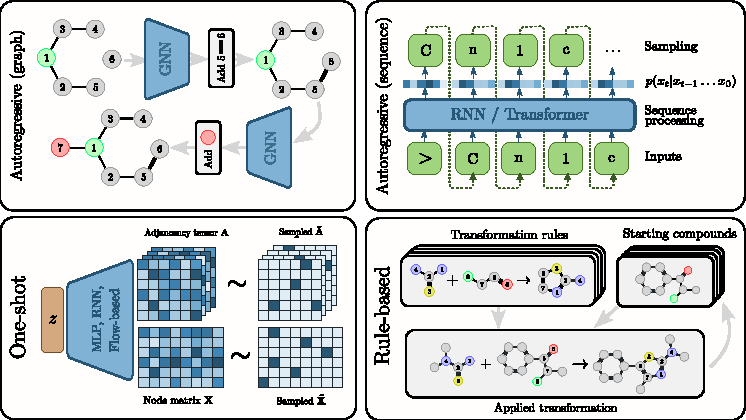
\includegraphics[width=\textwidth]{figures/generation_strategies_tryout.pdf}
    \caption{Different approaches to generate molecules in drug discovery. \textbf{A:} Graph-based
        autoregressive models generate molecules by iteratively adding nodes and edges to the
        graph, often relying on \acp{GNN} \textbf{B:} Sequence-based autoregressive models
        generate molecules by sampling one token at a time conditioned on the previously sampled
        tokens. Based on \acp{RNN} or Transformers \textbf{C:} Matrix-based models generate an
        adjacency matrix and node feature matrix of a molecule, followed by a discretization
        step. \textbf{D:} Rule-based models generate molecules by applying a set of pre-defined
        graph transformation rules to iteratively combine a set of starting molecules.
        \label{fig:generation-strategies}}
\end{figure}

\textbf{Graph-based autoregressive models} work similarly to its sequence-based counterpart, but
instead of relying on a linearization of the molecule, they directly construct the graph
representation of the molecule. The model generates the molecular graph by iteratively adding nodes
and edges to it, often relying on \acp{GNN} to decide which to add next. These models are more
complex as sequence-based autoregressive models as there is no prescribed order in which nodes and
edges are added to the graph \citep{hanFittingAutoregressiveGraph2023}. Notable examples of
graph-based autoregressive models for molecule generation include
\citep{liuConstrainedGraphVariational2018,liLearningDeepGenerative2018,youGraphConvolutionalPolicy2019,cohen-karlikOvercomingOrderAutoregressive2024}.

% Todo: Maybe add a bit more here
\textbf{Matrix-based models}  generate molecules by constructing a node feature matrix and an
adjacency tensor. The node feature matrix encodes which atoms are present in the molecule and the
adjacency tensor encodes the bonds and their types. Commonly a continuous version of the molecule is
generated first, with the entries in the matrices encoding probabilities of which atoms and bonds
will be present in the molecule. The continuous representation is then discretized to obtain a final
molecular graph, by sampling from the predicted probabilities. Some notable examples of
matrix-based models include \citep{simonovskyGraphVAEGenerationSmall2018,decaoMolGANImplicitGenerative2018,madhawaGraphNVPInvertibleFlow2019}.

% https://www.frontiersin.org/journals/hematology/articles/10.3389/frhem.2024.1305741/full#h4
\textbf{Rule-based models} generate molecules by applying a set of pre-defined graph transformation
rules to combine a set of starting compounds. By iteratively applying these rules, these models are
able to generate a wide range of molecular structures. The BRICS \citep{degenArtCompilingUsing2008}
method provides a set of molecular fragments and rules how to meaningfully combine them.
\citet{jensenGraphbasedGeneticAlgorithm2019} defines graph mutation and crossover operations to
generate new molecules, which are then used in the context of molecule optimization.
Transformation rules are well-suited to describe chemical reactions. The DOGS method
\citep{hartenfellerDOGSReactionDrivenNovo2012} generates new molecules by applying chemical reaction
rules to a set of starting molecules, which allows the generation of new molecules with known
synthetic routes. Rule-based models are often combined with machine learning models to predict the
outcome of chemical reactions
\citep{seglerNeuralSymbolicMachineLearning2017,seglerPlanningChemicalSyntheses2018,fortunatoDataAugmentationPretraining2020,daiRetrosynthesisPredictionConditional2020}.


\subsection{Distribution-learning}
\begin{figure}
    \centering
    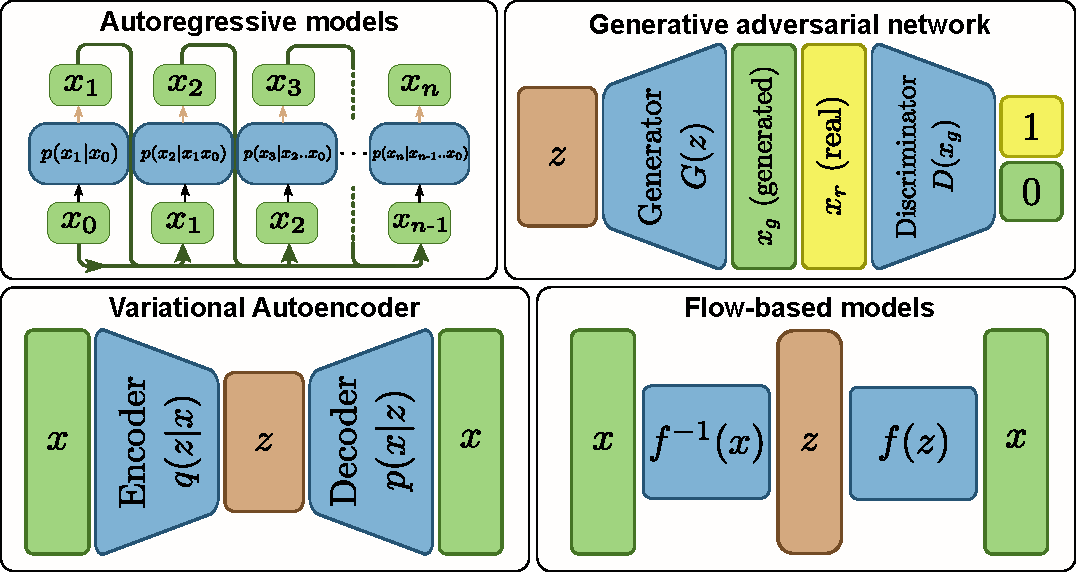
\includegraphics[width=0.99\textwidth]{figures/distribution-learning-models.pdf}
    \caption{Different types of distribution-learning models. All model types
        try to fit the data distribution, but differ in the way they achieve this goal.
        While for autoregressive models and generative flows the exact likelihood of the data can be calculated,
        and optimized, \emph{VAEs} rely on a variational approximation of the likelihood. Generative adversarial networks
        indirectly fit the data distribution using a game-theoretic approach. \label{fig:distribution-learning-models}}
\end{figure}
% Whats distribution learning
Distribution-learning is a fundamental application of generative models in \ac{DNDD}. Its
objective is to create a model that captures the distribution of molecules within a dataset and is
able to sample new molecules from it. These models can be trained in a self-supervised manner on
large chemical libraries of stable molecules, such as PubChem
\citep{kimPubChemSubstanceCompound2016}, ChEMBL \citep{bentoChEMBLBioactivityDatabase2014} or ZINC
\citep{irwinZINCFreeTool2012}. Using this process the resulting models can learn what reasonable
molecules look like in the context of drug discovery and learn the syntax of the selected molecular
representation. This makes them useful for their two main purposes: they can expand virtual
libraries and, more importantly, serve as a foundation for other applications such as goal-directed
generation, which we will explore in the next section.

In recent years, many new model architectures and training algorithms based on \ac{DL} have been
developed for distribution-learning. A majority of these were originally proposed for text and
image generation, but have been adapted to generate molecules. While all of them aim to approximate
the data distribution, they differ in the way they model the distribution and the choice of
molecular representation.

\textbf{Autoregressive models} make use of the chain rule of probability to factorize the likelihood
of a molecule into a product of conditional probabilities of the individual tokens. This model type
is trained by maximizing the likelihood of the training data with respect to the model parameters.
Autoregressive models are explicit density models, as the likelihood of sampling a molecule can be
calculated exactly, which facilitates model evaluation. Models trained in this way form the backbone
of many generative models in drug discovery
\citep{gomez-bombarelliAutomaticChemicalDesign2018,seglerGeneratingFocusedMolecule2018,olivecronaMolecularDenovoDesign2017,guoAugmentedMemoryCapitalizing2023,thomasAugmentedHillClimbIncreases2022,jaquesSequenceTutorConservative2016,cohen-karlikOvercomingOrderAutoregressive2024}.

\Acp{VAE} \citep{kingmaAutoEncodingVariationalBayes2013} generate molecules by first sampling from a
simple latent distribution and then mapping those latent samples to molecular space via a
probabilistic decoder network. To make training tractable, a second network, the encoder network is
used to map molecules back to the latent space. The model is then trained to maximize the \ac{ELBO}
of the data.
% \begin{align}
%       \log p(x) \geq \mathbb{E}_{q(z|x)}[\log p(x|z)] - \text{KL}(q(z|x) || p(z)),
% \end{align}
% where KL is the Kullback-Leibler divergence.
This model type has the advantage of providing a continuous latent space, which can be used to
interpolate between molecules and allows for use of continuous molecule optimization algorithms.
\acp{VAE} belong in the class of approximate density models, as the likelihood of
given molecule is given approximately the \ac{ELBO}. \acp{VAE} have been a
popular choice for generating molecules
\citep{gomez-bombarelliAutomaticChemicalDesign2018,kusnerGrammarVariationalAutoencoder2017,simonovskyGraphVAEGenerationSmall2018,samantaNeVAEDeepGenerative2018,jinJunctionTreeVariational2018,daiSyntaxDirectedVariationalAutoencoder2018,liuConstrainedGraphVariational2018}.

\textbf{Generative flows} \citep{rezendeVariationalInferenceNormalizing2016} transform a simple
latent space distribution into the data distribution via a sequence of invertible transformations
parameterized by neural networks. This makes it possible to calculate the likelihood of a given
molecule using the change of variables formula of probability. Similarly to autoregressive models,
generative flows are explicit density models, and are optimized by maximizing the likelihood of the
training data. Originally generative flows have been proposed for continuous data, but have been
adapted the discrete modality of graphs
\citep{madhawaGraphNVPInvertibleFlow2019,satorrasEquivariantNormalizingFlows2022,shiGraphAFFlowbasedAutoregressive2020,kuznetsovMolGrowGraphNormalizing2021}.
Similarly to \acp{VAE}, generative flows provide a continuous latent space, which can be used for
molecule optimization.
% p(x), via a bijective mapping $f: z \rightarrow x$. The likelihood of the training data can then be
% directly calculated and optimized via the change of variables formula:
% \begin{align}
%       p_x(x) = p_z(f^{-1}(x)) \left|
%       \det \left[
%       \left. \frac{\partial f^{-1}(v)}{\partial v} \right|_{v=x}
%       \right]
%       \right|.
% \end{align}

% molgan
\Acp{GAN} \citep{goodfellowGenerativeAdversarialNetworks2014} are latent space models that map a
simple distribution in latent space to molecular space, but rely on a game-theoretic approach to
training. A generator network is trained to generate data, which is then fed to a discriminator
network along with real data. The two networks then engage in a minimax game, where the
discriminator is trained to distinguish between real and generated data, while the generator is
trained to generate samples that fool the discriminator. Using this approach, \acp{GAN} can generate
realistic samples, but are harder to train and evaluate than other models. \Acp{GAN} are implicit
density methods as they only enable sampling from the model distribution, but do not provide
likelihoods for given samples. This approach has been combined with different generation strategies
in the context of drug discovery
\citep{decaoMolGANImplicitGenerative2018,kadurinDruGANAdvancedGenerative2017,guimaraesObjectiveReinforcedGenerativeAdversarial2017,mendez-lucioNovoGenerationHitlike2018,tangMolecularGenerativeAdversarial2024}.
\acp{GAN} also provide a continuous latent space but in contrast to \acp{VAE} and generative flows,
the latent code of a given molecule cannot be calculated, as no inverse mapping is given.

\subsection{Goal-directed molecule generation}
\begin{figure}
    \centering
    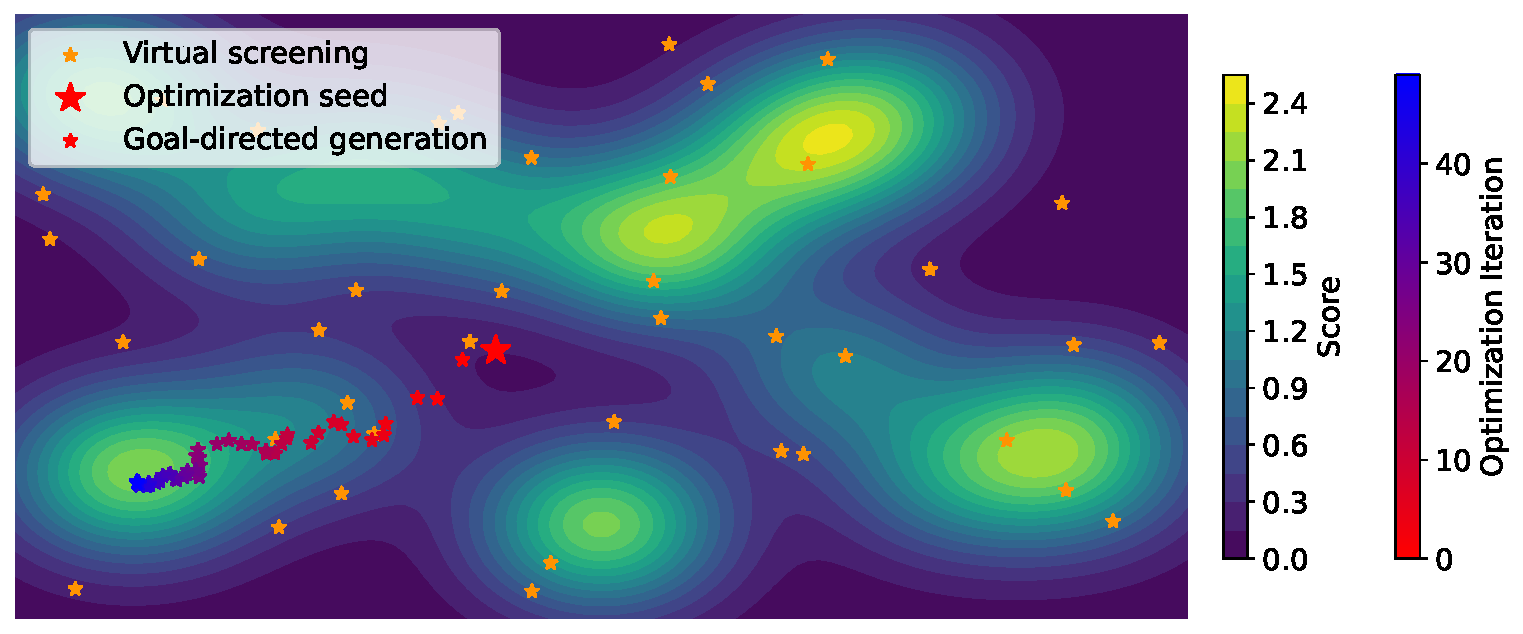
\includegraphics[width=0.8\textwidth]{./figures/goal_directed_generation_vs.pdf}
    \caption{Illustration of the difference between goal-directed molecule generation and virtual
        screening in a 2D chemical space, where each point in space corresponds to a molecule. The
        background color represents the molecules' scores. Goal-directed generation works
        akin to a numerical optimization algorithm and efficiently finds high-scoring molecules,
        shown in the transition from red to blue stars. In contrast, VS amounts to a random search in chemical space, which is less efficient
        and is likely to miss high-scoring regions of chemical space. \label{fig:goal-directed-generation}}
\end{figure}

% Whats goal-directed generation
Goal-directed molecule generation is a computational approach for automatically designing molecules
with desired property profiles. The desired property profile can either be a single molecular
property or a combination of multiple ones. In this thesis we assume that we are always given a
weighted combination of all properties of interest, resulting in scoring functions that assign
scalar values to molecules. The aim of goal-directed generation is to find molecules with the
highest possible score.

% why is VS not enough
Goal-directed generation expands upon \ac{VS}, which searches for molecules with the desired profile
in an existing library of molecules.\ \citet{waltersVirtualChemicalLibraries2019} estimates that approximately
$10^{13}$ molecules can be routinely tested in a \ac{VS} experiment. While this number can vary
significantly depending on the computational cost of evaluating the scoring function, it is dwarfed
by the size of drug-like chemical space, which is estimated to contain between $10^{30}$ and
$10^{60}$ molecules \citep{waltersVirtualChemicalLibraries2019,ruddigkeitEnumeration166Billion2012}.
Consequently, \ac{VS} is limited to exploring only a small fraction of chemical space and cannot
fully leverage the vast number of possible candidates that drug-like chemical space offers.

% How does goal-directed help and work
Goal-directed generators address this limitation of \ac{VS} by conducting a directed search in chemical
space. In contrast to the random search approach taken by \ac{VS},
goal-directed generators act more like optimizers that are able to efficiently locate maxima as
illustrated in \Cref{fig:goal-directed-generation}. This is achieved by an iterative process in
which a model generates a set of molecules, which are then scored by a \ac{QSPR} model. These scores
are then used to update the model, shifting the sampling distribution to regions of chemical space
with higher scores.

% Increased interest and different methods.
Recently, there has been a surge of deep learning-based goal-directed generators
\citep{eltonDeepLearningMolecular2019,sanchez-lengelingInverseMolecularDesign2018,duMachineLearningaidedGenerative2024}.
A multitude of different models has been proposed, which are based on a variety of neural network
architectures, training strategies and molecular representations. These methods augment traditional
rule-based generation approaches that have been combined with graph search and evolutionary
algorithms \citep{schneiderComputerbasedNovoDesign2005,schneiderNovoMolecularDesign2013}. This new
wave of \ac{DL} methods has shown promise in generating novel molecules with desired
property profiles and has seen use in a variety of applications, such as the design of new drugs,
materials or catalysts \citep{zhavoronkovDeepLearningEnables2019,anstineGenerativeModelsEmerging2023,zahrtPredictionHigherselectivityCatalysts2019,daveAutonomousDiscoveryBattery2020,kimDatadrivenElectrolyteDesign2023,moonActiveLearningGuides2024}.

Some of the most commonly used approaches to goal-directed molecular generation are:
\begin{itemize}
    \item \textbf{Hill-climbing}
          \citep{seglerGeneratingFocusedMolecule2018,xieMARSMarkovMolecular2021,thomasAugmentedHillClimbIncreases2022}
          is a simple optimization algorithm that relies on an underlying distribution-learning model.
          Molecules are sampled from the model's distribution and their scores are evaluated.
          The model is then retrained on the top-scoring molecules and the process is repeated.
    \item \textbf{Reinforcement learning} works similarly, but instead uses the scores of
          generated molecules as a reward signal to update the model distribution. This is
          achieved through methods based on the REINFORCE algorithm
          \citep{williamsSimpleStatisticalGradientfollowing1992} which allows updating the model
          distribution in a way that increases the scores of the generated molecules
          \citep{olivecronaMolecularDenovoDesign2017,thomasAugmentedHillClimbIncreases2022,youGraphConvolutionalPolicy2019,guoAugmentedMemoryCapitalizing2023}.
    \item \textbf{Genetic algorithms} evolve an initial population of molecules through iterative
          cycles of mutation, crossover, and selection
          \citep{jensenGraphbasedGeneticAlgorithm2019,nigamGenerativeModelsSuperfast2021,yoshikawaPopulationbasedNovoMolecule2018}.
          Starting from an initial set of molecules, new molecules are generated by applying random
          modifications. The molecules are then scored, and the best ones are selected for the
          next generation. This process is repeated for multiple generations, gradually optimizing
          the population towards desired molecular characteristics.
    \item \textbf{Tree search} methods build a tree of possible molecules by recursively applying a set of transformation rules
          to an initial set of molecules. Using techniques such as Monte Carlo Tree Search, the tree is
          explored to find the most promising molecules \citep{yangChemTSEfficientPython2017,jensenGraphbasedGeneticAlgorithm2019}.
    \item \textbf{Continuous optimization} methods employ classical optimization algorithms in the
          continuous latent space of (variational) autoencoders
          \citep{gomez-bombarelliAutomaticChemicalDesign2018,kusnerGrammarVariationalAutoencoder2017,winterEfficientMultiobjectiveMolecular2019},
          generative flows \citep{madhawaGraphNVPInvertibleFlow2019} or others. If the scoring
          function can be evaluated in the continuous space, it is possible to perform direct
          optimization, without the need for sampling the molecular graph.
    \item \textbf{Generative Flow Networks} \citep{bengioFlowNetworkBased2021} aim to generate
          molecules with probability proportional to their score. This method relies on an
          iterative generation process and models chemical space as a directed acyclic graph, with
          nodes representing intermediate molecules and edges representing graph edits. The transition
          probabilities between nodes are given by a "flow" of probability mass. The flow arriving
          at finished molecules, determines their probability of being sampled. The flows are
          then adjusted such that the final probability of a molecule being sampled is
          proportional to its score. This leads to the advantage of being able to explore multiple
          modes of the scoring function resulting in diverse solutions.
\end{itemize}

\subsection{Challenges in evaluating generative models in de novo design}
% Applications of Deep Learning in Molecule Generation and Molecular Property PredictionArticle link copied!

The evaluation of generative models is a challenging, as generative problems usually allow for a
range of valid solutions. This makes it hard to define a single ground truth solution, on which model
evaluation usually relies. In this section we discuss some of the challenges in evaluating
generative models in the context of de novo design.

\subsubsection{Evaluation of distribution-learning models}
The most basic and commonly used checks to assess the performance of distribution-learning models
are the validity, uniqueness and novelty of the generated molecules. A molecule is valid if it obeys
chemical valence rules, which is usually checked using chemoinformatics toolkits such as RDKit
\citep{landrumRDKitOpensourceCheminformatics2006}. The uniqueness of a set of molecules measures the
fraction of unique molecules in the set and can flag models that output many duplicates. The novelty
of a set of generated molecules is the fraction of generated molecules that are not in the training
set and can, to a certain extent, detect whether a model overfits to the training set.

A variety of approaches exists to assess how well a model can learn the distribution of the training
set. Explicit/approximate density models allow principled evaluation based on the likelihood on a
hold-out test set. However, this is not applicable to implicit density models such as \acp{GAN}.
Instead, the KL-divergence between the distributions of scalar molecular properties (e.g. molecular
weight or logP) of the generated molecules and the training set is commonly used to evaluate the
distribution fit \citep{brownGuacaMolBenchmarkingModels2019,polykovskiyMolecularSetsMOSES2020}.
However, this metric is usually determined using a limited number of properties and does not capture
correlations between them. The \ac{FCD} \citep{preuerFrechetChemNetDistance2018}
provides a more comprehensive evaluation, by comparing the distributions of the activations of a
neural network trained to predict bioactivities and has been shown to be sensitive to distributional
differences in many molecular properties.

The MOSES \citep{polykovskiyMolecularSetsMOSES2020} and GuacaMol
\citep{brownGuacaMolBenchmarkingModels2019} benchmarks add to these metrics and provide standardized
frameworks for evaluating distribution-learning models in molecular generation. While these
benchmarks represent progress, questions remain about their comprehensiveness and ability to fully
capture the complexity of performance evaluation.

\subsubsection{Goal-directed optimization of ML-based scoring functions}
\ac{ML} models have shown promise in predicting molecular properties
\citep{mayrDeepToxToxicityPrediction2016,klambauerMachineLearningDrug2019,vamathevanApplicationsMachineLearning2019,chenRiseDeepLearning2018,stokesDeepLearningApproach2020},
which makes them an attractive target for goal-directed generation. However, the fact that these
\ac{ML} models are often trained on limited amounts of experimental data, adds additional aspects
to a proper model evaluation. In this setting, there already are known molecules with high scores
that were used to train the scoring function. The task thus becomes finding novel
high-scoring molecules that differ from the training data. \ac{ML} models, however, are
often biased towards their training data, which might lead to a lack of novelty in the generated
molecules.

Furthermore, it has been shown that optimizing an \ac{ML} model's output with respect to its input
can lead to generated samples that incorrectly receive high scores
\citep{szegedyIntriguingPropertiesNeural2014,goodfellowExplainingHarnessingAdversarial2015}. This
can happen when the optimization algorithm leaves the applicability domain of the model, where the
scoring function is no longer reliable, but scores can still be high. Especially for scoring
functions trained on small datasets, the probability that the model drifts outside the applicability
domain is high. While this effect was initially studied in the image domain, where human vision can
easily provide ground truth evaluation, it is more challenging to identify this effect in molecular
optimization.

The extent of these biases, and their impact on the novelty of generated molecules are unknown, and it is
not clear how to quantify them without web-lab validation.

\subsubsection{Diversity of generated molecules}
Generating diverse sets of high-scoring molecules can increase the success chances of a drug
discovery project
\citep{martinDiverseViewpointsComputational2001,gorseDiversityMedicinalChemistry2006}. Having
multiple high-scoring molecules provides some insurance against the uncertainties and incomplete
scope of the scoring function and conducted experiments. Given that it is expected for some of
the generated molecules to fail in downstream testing, it is important to have a multitude of
candidates. Diversity among the candidates encourages uncorrelated outcomes in downstream testing, which
increases the chances of finding at least one successful candidate. In essence, a varied molecular
portfolio serves as a hedge against the inherent uncertainties in the modeling and experimental
outcomes.

% Bad diversity metrics
The concept of diversity in molecular generation is complex, with some of the most commonly used
diversity metrics being inadequate for goal-directed generation. The arguably most popular diversity
metric in the context of molecular generation is internal diversity
\citep{benhendaChemGANChallengeDrug2017}, which measures the average pairwise distance between
molecules. However, this metric is inadequate in the context of goal-directed generation
\citep{waldmanNovelAlgorithmsOptimization2000,xieMARSMarkovMolecular2021,thomasComparisonStructureLigandbased2021}.
\citet{thomasComparisonStructureLigandbased2021} proposed the \ac{SEDiv} metric, which aligns better
with chemical intuition but can be misleading when comparing sets of different sizes.

\citet{xieHowMuchSpace2023} recently addressed these shortcomings and introduced the \#Circles
metric which better reflects the requirements of evaluating goal-directed generators. \#Circles is a
non-normalized version of \ac{SEDiv} and provides an absolute measure of the chemical space covered
by the generated molecules. It is motivated by an axiomatic approach similar to the one used in
\citep{waldmanNovelAlgorithmsOptimization2000} and has been shown to correlate better with the
functional diversity of the generated molecules. Initial evaluations of goal-directed
generators using \#Circles have been conducted, but are limited by the fact
that the tested models were not adapted to the diverse optimization setting and not
tested under controlled computational budgets.

A comprehensive comparison of models specifically designed for diverse optimization is still
missing, leaving open the question of how well various approaches perform in generating diverse,
high-scoring molecules.

\subsubsection{Standardized Computational Resources}
A frequently neglected aspect in evaluating goal-directed models is the use of standardized
computational resources. At its core, goal-directed generation is a search problem
that, given infinite resources, can be solved through exhaustive enumeration of drug-like chemical space.
Consequently, the primary challenge in goal-directed generation lies in identifying high-scoring molecules
within reasonable computational constraints.

% Current literature
However, many studies compare different models without accounting for this crucial factor,
potentially leading to biased comparisons. This might lead to scenarios where generators running for
days are compared to models that run for minutes, thereby leading to unfair comparisons. Recently,
this issue has gained increased attention after \citep{gaoSampleEfficiencyMatters2022} proposed a
benchmark that measures the sample efficiency of goal-directed generation algorithms, arguing that
in practical applications the bottleneck is the number of scoring function evaluations that can be
performed. Other researchers have adapted to this approach
\citep{thomasReevaluatingSampleEfficiency2022,thomasAugmentedHillClimbIncreases2022,guoAugmentedMemoryCapitalizing2023},
putting a stronger emphasis on controlling for computational budgets.

However, sample efficiency is most relevant when using scoring functions that are expensive to
evaluate. In many cases, the cost of evaluating the scoring function is on the same order of
magnitude or smaller than the cost of generating the molecules. In this case, different
computational constraints need to be used to account for both the generation and scoring of
molecules. Consequently, there is a need for a more comprehensive evaluation framework for
goal-directed generation models that controls for various types of computational budgets, especially
in the context of finding diverse high-scoring molecules.

% Cross check with the paper
\subsection{Retrosynthesis prediction}
% Add figure of search tree 
Drug candidates, whether designed by generative models or other means, need to be
synthesized for testing and eventually for use in patients. However, finding a synthesis route for a
given molecule can be a complex and time-consuming process. \Ac{CASP} methods help
chemists to find synthesis routes, enabling synthesis of previously inaccessible molecules or making
synthesis more efficient and cost-effective.

This problem is often approached using a retrosynthesis approach
\citep{coreyComputerAssistedDesignComplex1969,coreyLogicChemicalSynthesis1991a}, which
recursively deconstructs the target molecule into simpler precursors until they match available
starting materials. At each step, single-step retrosynthesis prediction models suggest sets of
reactants that could theoretically combine to produce the current, intermediate molecule.
The success of retrosynthesis planning hinges on highly accurate chemical reaction models, as these
ensure that the proposed synthetic routes are actually feasible.

Early work in retrosynthesis prediction relied on carefully curated expert rules encoding possible
reactions. Recently, machine learning models that learn the patterns of chemical reactions from
examples stored in reaction databases have received increased attention
\citep{coleyMachineLearningComputerAided2018,strieth-kalthoffMachineLearningRopes2020}. One line of
work relies on sequence-to-sequence models originally developed for machine translation, to predict
the SMILES strings of reactants given the SMILES string of the target molecule
\citep{schwallerMolecularTransformerModel2019,namLinkingNeuralMachine2016,schwallerFoundTranslationPredicting2018,karpovTransformerModelRetrosynthesis2019,tetkoStateoftheartAugmentedNLP2020}.
Another set of approaches exploits the fact that connectivity in a reaction is often highly
preserved, and use graph neural networks to edit the connectivity of the target molecule in order to
yield possible reactants
\citep{sachaMoleculeEditGraph2020,shiGraphGraphsFramework2020,somnathLearningGraphModels2020,yanRetroXpertDecomposeRetrosynthesis2020}.

Template-based methods represent another approach to retrosynthesis prediction
\citep{seglerNeuralSymbolicMachineLearning2017,seglerPlanningChemicalSyntheses2018,daiRetrosynthesisPredictionConditional2020,sunEnergybasedViewRetrosynthesis2020}.
These models rely on a set of graph transformation rules, or templates, that encode the connectivity
changes that occur in a reaction. These templates can either be extracted from reaction databases or
be hand-coded by chemists. To predict which templates are most likely to yield feasible reactions,
\ac{ML} models are trained on examples of recorded chemical reactions. The trained model can then be
in multistep algorithms to plan synthesis routes for molecules of interest.

While template-based methods have shown excellent performance in retrosynthesis prediction, they
face challenges with rare templates. Template extraction from databases often leads to many
templates being represented by only a few training samples
\citep{fortunatoDataAugmentationPretraining2020}, resulting in a challenging few-shot learning
problem. While some strategies have been proposed to alleviate this issue, such as data augmentation
\citep{fortunatoDataAugmentationPretraining2020} and specialized architectures and training
objectives \citep{daiRetrosynthesisPredictionConditional2020}, the problem remains a challenge in
the field.

\section{Contributions\label{sec:contributions}}
\subsection{Identifying failure modes in generative model evaluation}
In \citep{renzFailureModesMolecule2019} we investigate possible failure modes in the evaluation of
distribution-learning and goal-directed generative models. We show that the distribution-learning
benchmark proposed in GuacaMol \citep{brownGuacaMolBenchmarkingModels2019} is not able to
distinguish recently published generative models from a simple baseline model. The tested generative
models either underperform or only marginally outperform the baseline model, calling for a more
comprehensive evaluation of distribution-learning models.

Furthermore, we introduce control scores to detect overfitting of goal-directed generators to
\ac{ML}-based scoring functions. Testing various generators with these control scores reveals that
generated molecules are biased towards high-scoring molecules in the training set, resulting in
limited novelty. Additionally, generative models overfit to artifacts of the scoring function
leading to overestimation of performance. \Cref{sec:failure-modes} reprints the corresponding
publication.

\subsection{Diversity-based comparison of goal-directed generators\label{sec:divopt}} In
\citep{renzDiverseHitsNovo2024} we introduce a benchmark for diverse optimization that addresses the
above-mentioned issues. In this benchmark, we evaluate the diversity of the generated molecules
using the recently proposed diversity metric \#Circles \citep{xieHowMuchSpace2023}. We compare the
performance of diverse optimization approaches under two different compute budgets, namely a fixed
number of scoring function evaluations and a fixed time budget. We use this setup to benchmark a
range of established goal-directed generators, adapted to diverse optimization using the diversity
filter introduced in \citep{blaschkeMemoryassistedReinforcementLearning2020}.
\Cref{sec:diverse-hits} reprints the corresponding publication.

\subsection{Improving few-shot and zero-shot retrosynthesis prediction}
In \citep{seidlImprovingFewZeroShot2022} we propose a novel approach to template-based
retrosynthesis prediction. We use a multimodal learning approach that learns to associate relevant
templates to product molecules using a Modern Hopfield Network
\citep{ramsauerHopfieldNetworksAll2020}. In contrast to previous template-based methods, our model
processes the structure of templates and can make use of similarities between them. We achieve
state-of-the-art performance in single-step retrosynthesis prediction, and perform particularly well
for templates with few training samples. Our model achieves high inference speeds while maintaining
good predictive performance. \Cref{sec:mhn-react} reprints the corresponding publication.

\section{List of publications\label{sec:publications}} This thesis comprises the work published in
the following papers:

\begin{itemize}
    \item \printpublication{renzFailureModesMolecule2019}
    \item \printpublication{renzDiverseHitsNovo2024}
    \item \printpublication{seidlImprovingFewZeroShot2022}
\end{itemize}

% give overview over my other publications
\paragraph{Other Publications} Besides the papers listed above, I have also contributed to the
following publications:

\begin{itemize}
    \item \printpublication{preuerFrechetChemNetDistance2018}
    \item \printpublication{renzUncertaintyEstimationMethods2019}
    \item \printpublication{hofmarcherLargescaleLigandbasedVirtual2020}
    \item \printpublication{renzLowCountTimeSeries2023}
\end{itemize}